% Informe final OII464. Formato institucional de la Escuela de Ingeniería
% Informática PUCV y propuesta de selección adaptativa de movimientos.
\documentclass[12pt,letterpaper]{report}
\usepackage[spanish,es-nodecimaldot]{babel}
\usepackage{pucv_inf_2024}
% Cifras en modo matemático con la misma Times del texto.
\usepackage{mathptmx}
\usepackage{amssymb,booktabs,array,microtype,csquotes}
\usepackage[hidelinks]{hyperref}
\addbibresource{referencias.bib}
\DefineBibliographyExtras{spanish}{\protected\def\bibrangedash{\textendash\penalty\hyphenpenalty}}
\renewcommand{\thesection}{\arabic{section}}
\renewcommand{\thesubsection}{\thesection.\arabic{subsection}}
\renewcommand{\thetable}{\arabic{table}}
\renewcommand{\thefigure}{\arabic{figure}}
\renewcommand{\thealgorithm}{\arabic{algorithm}}
\captionsetup[table]{name=Tabla}
\captionsetup[figure]{name=Figura}
\addto\captionsspanish{\renewcommand{\contentsname}{Índice}}
\algrenewcommand\algorithmicrequire{\textbf{Entrada:}}
\algrenewcommand\algorithmicfor{\textbf{para}}
\algrenewcommand\algorithmicwhile{\textbf{mientras}}
\algrenewcommand\algorithmicdo{\textbf{hacer}}
\algrenewcommand\algorithmicif{\textbf{si}}
\algrenewcommand\algorithmicthen{\textbf{entonces}}
\algrenewcommand\algorithmicelse{\textbf{si no}}
\algrenewcommand\algorithmicend{\textbf{fin}}
\algrenewcommand\algorithmicreturn{\textbf{devolver}}
\setlength{\headheight}{14pt}
\hypersetup{
 pdftitle={Programación de cirugías electivas mediante búsqueda tabú y selección adaptativa de movimientos},
 pdfauthor={José Basualto, Cristopher Dauros, Carlos Ruz},
 pdfsubject={Informe final del proyecto OII464},
 pdfkeywords={programación de cirugías, búsqueda tabú, selección adaptativa de operadores, aprendizaje en línea}
}

\begin{document}
\hypersetup{pageanchor=false}
% Adaptación de la portada para asignaturas de la plantilla PUCV 2024.
\title{Programación de cirugías electivas\\[0cm]
mediante búsqueda tabú y selección\\[0.2cm]
adaptativa de movimientos}
\author{José Basualto, Cristopher Dauros y Carlos Ruz}
\date{22 de noviembre de 2026}

\begin{titlepage}
  \makeatletter
  \thispagestyle{empty}
  \begin{picture}(0,0)
    \put(-75,-80){
\includegraphics[width=20cm]{Portadas/imagenes/encabezado.png}}
  \end{picture}
  \begin{flushright}
    \vspace*{\fill}
    {\textcolor{titlecolor}{\LARGE\bfseries\MakeUppercase{\\[3cm]\@title}}}
    \vspace*{\fill}

    {\textcolor{titlecolor}{\Large\bfseries\scshape
      \begin{tabular}{@{}r@{}}
        José Basualto\\[0.2cm]
        Cristopher Dauros\\[0.2cm]
        Carlos Ruz
      \end{tabular}}}\\[1cm]
    {\textcolor{titlecolor}{\bfseries\textsc{
      Informe final\\[0.2cm]
      OII464: Desarrollo de Diseños Híbridos para Optimización\\[0.2cm]
      \@date}}}
  \end{flushright}
  \makeatother
\end{titlepage}

\hypersetup{pageanchor=true}
\pagenumbering{arabic}

\chapter*{Resumen}
La programación de cirugías electivas coordina anestesia y cirugía con recursos
que se bloquean si el paciente espera entre etapas. Aunque existen híbridos con
selección adaptativa de operadores, falta establecer cuánto aporta esta a una
búsqueda tabú con espera estricta y reparación. Proponemos que un bandido
multibrazo dinámico (D-MAB) aprenda en línea qué movimiento proponer, dentro de una
cartera con una búsqueda tabú uniforme. Contribuimos con controles que separan
selección adaptativa, presupuesto, repetición de la búsqueda y reinicio
Page--Hinkley. Lo evaluamos en 48 instancias sintéticas congestionadas, derivadas de
las 12 oficiales, con 20 semillas, Wilcoxon e intervalos de 95~\%. Frente a la
selección uniforme, D-MAB obtuvo una diferencia no concluyente de $-0{,}793$
unidades del objetivo (IC [$-1{,}850$; $+0{,}279$]). La cartera superó a la
búsqueda prolongada ($-1{,}380$), pero no se distinguió de dos búsquedas independientes; además,
UCB1 sin reinicio superó a D-MAB por 1,824. Al reanalizar de forma exploratoria por instancia base,
ambas ventajas perdieron significación. Sí se mantuvo una confirmación
prerregistrada con semillas nuevas: UCB1 superó a la selección uniforme
($-2{,}749$; IC [$-4{,}069$; $-1{,}453$]). Así, la evidencia favorece a UCB1 bajo
congestión, pero no fue consistente en el catálogo oficial.
% fuente: secciones 4.2 a 4.6

\noindent\textbf{Palabras clave:} programación de cirugías; búsqueda tabú;
selección adaptativa de operadores; aprendizaje en línea; bloqueo.

\clearpage
\tableofcontents

\clearpage
\section{Introducción}
\label{sec:introduccion}\label{int-ini}
Organizar una jornada quirúrgica supone distribuir una capacidad limitada entre
pacientes con duraciones y requerimientos distintos. Los quirófanos, el personal
y los tiempos de preparación y limpieza condicionan el orden de atención y el
término de la jornada. Cuando la anestesia y la cirugía son etapas distintas, el
paciente puede esperar por la segunda sala o por el cirujano. Esa espera retiene
la primera sala y a su anestesista, lo que retrasa a los pacientes siguientes.
Por ello, el problema busca reducir el bloqueo y el \emph{makespan}, es decir, el
término de la última operación. Además, debe respetar la precedencia, la espera
máxima y la disponibilidad de recursos \parencite{lara2026}.

El aprendizaje puede intervenir en distintos puntos de una metaheurística.
\textcite{akbarzadeh2024} predicen la factibilidad de los cromosomas y
\textcite{niroumandrad2024} filtran movimientos de una búsqueda tabú con
clasificadores; ambos buscan reducir el esfuerzo de evaluación. En cambio, otros
trabajos aprenden qué operador aplicar. \textcite{yu2024} usan Q-learning en
programación quirúrgica, y el preprint de \textcite{dolatkhah2026} usa una variante
de D-MAB en un algoritmo genético que genera columnas iniciales. Sin embargo,
\textcite{yin2026} muestran que combinar operadores en una búsqueda tabú iterada
ya puede dar soluciones cercanas a cotas inferiores. Una mejora puede venir,
entonces, del vecindario y no del aprendizaje. A su vez, \textcite{dacosta2008}
fundamentaron D-MAB con recompensas artificiales, fuera de una búsqueda, y su
reinicio no fue superior en todos los escenarios. Por tanto, falta separar el
aporte de la política de selección del aporte de los operadores y del cómputo.

En los trabajos revisados no encontramos esa separación para una búsqueda tabú de
dos etapas con espera estricta y reparación. La reparación es relevante, porque
puede alterar el movimiento que recibe la recompensa. Además, un híbrido puede
parecer mejor solo por consumir más evaluaciones o por repetir la búsqueda. Por
ello, este proyecto pregunta en qué condiciones D-MAB mejora a una búsqueda tabú
frente a la selección uniforme de los mismos movimientos.

El objetivo es medir ese aporte en la calidad de las soluciones y describir su
costo y su robustez entre semillas. El híbrido combina una metaheurística (MH)
con aprendizaje automático (ML) en la fase de \emph{evolución}
\parencite{vega_taxonomia}. La evaluación usa las 12 instancias oficiales
\parencite{saicooh2026} y, como estudio principal, 48 instancias sintéticas con
congestión de cirujanos.
Atribuimos una mejora a la selección adaptativa solo si resiste los controles que no aprenden.
Ganar a una búsqueda más corta no basta, ni tampoco una ganancia que se iguale al
repetir la búsqueda. Del mismo modo, informamos los resultados desfavorables y las
condiciones en que la ventaja desaparece.

Las contribuciones son tres. Primero, una cartera fija que combina una trayectoria
con D-MAB y una trayectoria uniforme de referencia. Segundo, un diseño de controles
que separa política de selección, presupuesto, repetición y reinicio. Tercero, un catálogo
reproducible que tensiona la espera entre etapas.

La sección~\ref{sec:propuesta} presenta la propuesta y la
sección~\ref{sec:experimental}, el diseño experimental. Luego, la
sección~\ref{sec:resultados} discute los resultados y la
sección~\ref{sec:conclusion} responde la pregunta. En cada una declaramos los límites,
para no extender la respuesta más allá de las condiciones evaluadas. Así, el lector puede
distinguir lo confirmado, lo exploratorio y lo descriptivo.\label{int-fin}

\clearpage
\section{Propuesta metodológica}
\label{sec:propuesta}\label{pro-ini}
La idea central es que un bandido aprenda, durante cada corrida, qué movimiento
debe proponer una búsqueda tabú, en adelante Tabu. Una trayectoria uniforme
conserva una referencia sin aprendizaje. El Algoritmo~\ref{alg:cartera} resume
el flujo completo.

\subsection{Problema, representación y factibilidad}
La agenda es estática, con duraciones conocidas. La solución fija el orden y una
sala por etapa, mientras el planificador asigna al profesional elegible que se
libera primero. La espera y el fin de la jornada son
\begin{equation}
 W_j=\max\{0,T_j^C-F_j^A\},\qquad 0\leq W_j\leq L_j,
 \qquad C_{\max}=\max_{j\in J}F_j^C.
 \label{eq:restricciones}
\end{equation}
\noindent $J$ es el conjunto de pacientes y $j$, un paciente. $T_j^C$ es el
inicio de cirugía, posterior a su preparación. $F_j^A$ y $F_j^C$ son los fines de
cada etapa, incluida la limpieza. $W_j$ es la espera, $L_j$ su límite estricto y
$C_{\max}$ el \emph{makespan}. El anestesista queda reservado hasta que empieza la
cirugía. La primera sala también, salvo que sea la misma de la cirugía: en ese
caso se ocupa hasta el final. Esta regla sigue la formulación de clase
\parencite{lara2026}; el simulador estricto docente retiene la sala hasta el fin
de la cirugía (sección~\ref{subsec:amenazas}).

Se minimiza el criterio
\begin{equation}
 f(S)=C_{\max}+10^{-6}\sum_o t_o^{\mathrm{ini}}
        +0{,}5\sum_{j\in J}W_j+1{,}4\max_{j\in J}W_j,
 \label{eq:objetivo}
\end{equation}
\noindent donde $S$ es un calendario, $o$ una operación y $t_o^{\mathrm{ini}}$ su
inicio de reserva. El coeficiente $10^{-6}$ desempata. Los pesos 0,5 y 1,4 vienen de clase; omitimos su penalización por
desequilibrio de salas. Como $f$ es un criterio ponderado, una baja de $f$ no
implica la misma baja del \emph{makespan}.
% fuente: presentación del curso (Lara Arce, 2026), diapositivas 10 a 12; repositorio docente
% commit ecd30e3, simulation/scheduler.py (room_release) y config/config.yaml

Las claves aleatorias representan el orden y las salas. El decodificador pospone
a los pacientes que no caben sin violar la espera y elige las salas más parecidas
a las propuestas. Esta reparación puede alterar el movimiento, por lo que se
registra su frecuencia.

\subsection{Componente MH: búsqueda tabú}
Tabu \parencite{glover1989} parte de la mejor de 30 soluciones: FIFO (orden
original), SPT y LPT (duración total creciente y decreciente) y 27 aleatorias.
Sus cinco movimientos son intercambio, inserción y cambio de la sala de anestesia,
de cirugía o de ambas. Con probabilidad 0,65, el paciente a mover sale de los
tres con más espera positiva; en otro caso, se sortea entre todos. Cada iteración
evalúa hasta 15 candidatos distintos. La memoria guarda siete soluciones y admite
aspiración por mejora global. Si todo el lote es tabú, se acepta su mejor candidato.
% fuente: src/surgery_optim/tabu.py

\subsection{Componente ML: selección adaptativa en la evolución}
Cada movimiento es un brazo del bandido. UCB1 \parencite{auer2002} equilibra la
recompensa media $\bar r_a$ y la exploración de los brazos menos probados. Luego
de probar una vez cada brazo, elige
\begin{equation}
 a^*=\arg\max_a\Bigl[\bar r_a+c\sqrt{2\ln n/n_a}\,\Bigr],
 \qquad r=\min\Bigl\{1,\frac{\max\{0,f_{\mathrm{loc}}-f'\}}{\max\{1,\,0{,}02f_0\}}\Bigr\},
 \label{eq:bandido}
\end{equation}
\noindent donde $n_a$ cuenta los usos del brazo $a$, $n$ su suma y $c$ regula la
exploración. La recompensa $r$ compara al candidato reparado, de valor $f'$, con
el estado local del lote, $f_{\mathrm{loc}}$. Se escala con el objetivo inicial $f_0$. Un candidato repetido en el lote recibe cero y no consume evaluación.

D-MAB agrega a UCB1 la prueba de Page--Hinkley, que detecta caídas de la
recompensa \parencite{dacosta2008}. Tras actualizar $\bar r_a$, cada brazo acumula
$m_a\leftarrow m_a+r-\bar r_a+\delta$ y guarda su máximo $M_a$. Si
$M_a-m_a>\lambda$, se reinician las estimaciones de los cinco brazos, sin alterar
la memoria tabú. En este informe, UCB1 designa el mismo bandido sin ese reinicio.
% fuente: src/surgery_optim/bandit.py

\subsection{Orquestación y cartera con respaldo}
Fuera de línea se preparan las instancias y se fijan los parámetros. En línea,
cada camino genera, repara y evalúa candidatos. D-MAB aprende solo durante su
corrida, sin entrenamiento previo: decide qué vecino proponer, el planificador
asegura la factibilidad y Tabu elige el vecino aceptado.

\begin{algorithm}[!ht]
\footnotesize
\caption{Cartera de Tabu uniforme y Tabu con D-MAB.}
\label{alg:cartera}
\begin{algorithmic}[1]
\Require instancia, semilla y presupuesto $B=3.030$ por camino
\For{cada política $\pi\in\{\text{uniforme},\ \text{D-MAB}\}$}
  \State $S\gets$ mejor de las 30 iniciales; $e\gets 30$; memoria y bandido nuevos
  \While{$e<B$}
    \While{el lote tenga menos de 15 candidatos, $e<B$ y queden intentos}
      \State $a\gets$ movimiento elegido por $\pi$; $S'\gets$ reparar(mover($S$, $a$))
      \If{$S'$ ya está en el lote} $r\gets 0$
      \Else{} evaluar $S'$; $e\gets e+1$; calcular $r$ con la ecuación~\eqref{eq:bandido}
      \EndIf
      \State si $\pi$ es D-MAB, actualizar $a$ con $r$ y aplicar Page--Hinkley
    \EndWhile
    \State $S\gets$ mejor candidato admisible; actualizar la memoria y el mejor global
  \EndWhile
\EndFor
\State \Return el calendario factible de menor $f$ entre ambos caminos
\end{algorithmic}
\end{algorithm}

La cartera ejecuta ambos caminos en secuencia, con la misma instancia y semilla,
pero con memorias independientes. El criterio de parada es agotar 6.060
evaluaciones, 3.030 por camino, incluidas las iniciales. El reparto es fijo y no
aprende qué camino ganará. Por construcción, la cartera no empeora a ninguno de
sus dos caminos, aunque no garantiza superar a un Tabu de 6.060.

\subsection{Supuestos, datos y plan de evaluación}
Suponemos datos deterministas, disponibilidad completa del personal al inicio y
ausencia de urgencias. Los datos son sintéticos, sin identificadores clínicos.
El tamaño, los recursos y la espera permitida describen cada instancia, pero no
son entradas de D-MAB, que no usa contexto.

La evaluación mide $f$, sus componentes, la dispersión entre semillas, la desviación
relativa, el tiempo y la convergencia. Los controles son las reglas constructivas,
Tabu uniforme, Tabu prolongado, dos Tabu independientes y UCB1. No se compara
D-MAB contra la cartera completa, porque esta lo contiene y no puede ser peor. La
sección~\ref{sec:experimental} detalla el protocolo.\label{pro-fin}

\clearpage
% Sección (iv) Experimental Setup. Se inserta en main.tex antes de los Resultados:
%   \clearpage
%   % Sección (iv) Experimental Setup. Se inserta en main.tex antes de los Resultados:
%   \clearpage
%   % Sección (iv) Experimental Setup. Se inserta en main.tex antes de los Resultados:
%   \clearpage
%   \input{experimental_setup}
% Usa solo paquetes ya cargados por main.tex y pucv_inf_2024.sty.
% Referencia eq:objetivo, definida en la Propuesta metodológica.
% Describe el diseño. Los resultados están en la sección 4.
\section{Configuración experimental}
\label{sec:experimental}\label{set-ini}

La hipótesis primaria plantea que, bajo congestión, Tabu con D-MAB obtiene menor $f$
medio que Tabu uniforme. Fijamos hipótesis, semillas y pruebas en un protocolo
fechado en Git antes de ejecutar (31 de octubre de 2026, commit \texttt{a0da669}).
La confirmación E1 tuvo su propio protocolo (15 de noviembre, commit \texttt{05ca74a}).
El código, los protocolos y las corridas están en la rama \texttt{entrega3} del
\href{https://github.com/Josebasualto06/Cirugias-Tabu-DMAB-Entrega2-Jose./tree/entrega3}{repositorio del proyecto}:
{\footnotesize\url{https://github.com/Josebasualto06/Cirugias-Tabu-DMAB-Entrega2-Jose./tree/entrega3}}.

\subsection{Conjuntos de datos}
\label{subsec:datos}
Usamos dos catálogos sintéticos y los analizamos por separado. El estándar proviene
del repositorio oficial \parencite{saicooh2026}, con tres réplicas de 15, 20, 25 y
30 cirugías. Este catálogo casi no tensiona la espera: solo 16 de 240 soluciones
de la cartera terminaron con espera positiva.
% fuente: experiments/results/portfolios_60_79/runs.csv

Por ello, generamos un catálogo de congestión de 48 instancias, doce por tamaño,
cada una con semilla propia. El generador remuestrea pacientes de una instancia
estándar, aplica ruido lognormal con $\sigma=0{,}10$, redondea a 0,5 minutos y
sortea la elegibilidad del personal. Una calibración previa evaluó 18 combinaciones
de salas, cirujanos y espera máxima en cuatro instancias de desarrollo, excluidas
del catálogo. La regla prerregistrada exigía más de 50~\% de soluciones con espera
y eligió reducir los cirujanos al 40~\%, redondeando hacia arriba. No usó la
diferencia entre métodos. ML aprende en línea, por lo que no requiere partición de
entrenamiento.
% fuente: experiments/results/entrega2_calibracion_congestion_85_89/

\subsection{Líneas base, controles y métricas}
\label{subsec:controles}
La Tabla~\ref{tab:lineas-base} vincula cada control con la explicación alternativa
que evalúa. C1 a C4 son las comparaciones confirmatorias.

\begin{table}[!ht]
 \centering\footnotesize
 \caption{Controles y explicación alternativa que evalúa cada uno.}
 \label{tab:lineas-base}
 \begin{tabular}{@{}p{0.28\textwidth}p{0.24\textwidth}p{0.42\textwidth}@{}}
  \toprule
  Control (evaluaciones) & Comparación & Explicación alternativa\\
  \midrule
  FIFO, SPT y LPT & Descriptiva & Una regla constructiva basta.\\
  Tabu uniforme (3.030) & C1: D-MAB $-$ uniforme & La mejora es de Tabu y no de aprender.\\
  Tabu prolongado (6.060) & C2: cartera $-$ prolongado & La cartera solo usa más evaluaciones.\\
  Dos Tabu (6.060) & C3: cartera $-$ dos Tabu & La cartera solo repite la búsqueda.\\
  UCB1 (3.030) & C4: D-MAB $-$ UCB1 & El efecto es de UCB1 y no del reinicio.\\
  \bottomrule
 \end{tabular}
\end{table}

La métrica primaria es $f$. Por instancia calculamos mejor, media, peor y desviación
estándar (DE) entre semillas, y luego promediamos. La desviación relativa es
$\mathrm{RPD}=100(f-f^*)/f^*$, con $f^*$ como el mejor valor de la instancia en
nuestros dos estudios de congestión; no es un óptimo. También describimos
$C_{\max}$, esperas, factibilidad, tiempo de pared, propuestas decodificadas y
convergencia. Las métricas secundarias y los análisis por tamaño son descriptivos.
Los que no estaban en el protocolo se calcularon después y no cambian decisiones.

\subsection{Implementación y calibración}
\label{subsec:implementacion}
El código usa Python~3.13.2, NumPy~2.2.3, SciPy~1.15.2 y PyYAML~6.0.3. Los estudios de
congestión corrieron en un AMD Ryzen~7 8845HS de 8 núcleos, con 13,8~GiB de RAM y
Windows~11. Usaron procesos concurrentes; por eso, los tiempos solo se comparan dentro de un estudio.

\begin{table}[!ht]
 \centering\footnotesize
 \caption{Parámetros congelados, conteo del presupuesto y semillas.}
 \label{tab:parametros}
 \begin{tabular}{@{}p{0.13\textwidth}p{0.83\textwidth}@{}}
  \toprule
  Componente & Configuración\\
  \midrule
  Tabu & 30 iniciales; lotes de 15; hasta 150 intentos por lote; memoria de 7 soluciones; prioridad 0,65.\\
  Bandido & 5 brazos; $c=0{,}1$. Solo D-MAB: $\delta=0{,}01$ y $\lambda=1$.\\
  Cartera & Dos caminos de 3.030 evaluaciones; reparto 50/50; conserva el menor $f$.\\
  Conteo & Cuentan las iniciales y cada candidato distinto del lote, aun infactible. Los duplicados se decodifican, pero no cuentan. Tampoco la revalidación final.\\
  Semillas & 0--5: calibración. 20--39, 40--59 y 60--79: catálogo estándar. 85--89: calibración de congestión. 90--109: C1--C4. 110--114: piloto a igual tiempo. 115--119: diagnóstico. 120--139: E1. El segundo Tabu suma 1.000.000 a la semilla.\\
  \bottomrule
 \end{tabular}
\end{table}

La calibración comparó 14 variantes de política, memoria, $c$ y $\lambda$ en las
semillas 0--5 de las 12 instancias estándar. Elegimos la variante de D-MAB con menor
media frente a Tabu uniforme: $-0{,}224$, contra $-0{,}140$ de la siguiente, una
brecha menor que el ruido. UCB1 heredó $c$ para que C4 solo quite el reinicio. Los
demás parámetros de Tabu y $\delta$ se fijaron sin calibrar, y nada se recalibró
bajo congestión.
% fuente: experiments/results/calibration_0_5/ y entrega3_revision/descriptivos.csv

\subsection{Corridas y análisis estadístico}
\label{subsec:estadistica}
El diseño es pareado: cada método recibe las mismas 48 instancias y 20 semillas
(90--109), es decir, 960 corridas. C1 es la hipótesis primaria. C1 y C4 usan 3.030
evaluaciones; C2 y C3, 6.060. E1 compara UCB1 con Tabu uniforme en las semillas
120--139. Cada diferencia es alternativa menos referencia, así que un valor negativo
favorece a la alternativa.

La prueba de Wilcoxon bilateral \parencite{wilcoxon1945} opera sobre las medias por
instancia, con $\alpha=0{,}05$, y Holm \parencite{holm1979} corrige C1--C4. En E1 hay una
sola comparación, sin corrección. Los
intervalos de 95~\% usan una adaptación jerárquica del bootstrap
\parencite{efron1979}, que remuestrea instancias y semillas en 5.000 réplicas. Es
conservadora, porque las medias por instancia ya contienen ruido de semillas. La
regla exige $p<0{,}05$, intervalo bajo cero y media de a lo sumo $-0{,}25$.
Este umbral mínimo es la resolución de un paso de espera en $f$, no un umbral de
relevancia clínica.

\begin{table}[!ht]
 \centering\footnotesize
 \caption{Tamaños para potencia 0,80 y $\alpha=0{,}05$, según los 240 pares de las semillas 60--79. DE: de la diferencia. ED: efecto de diseño por agrupar en instancias, que multiplica los pares independientes.}
 \label{tab:potencia}
 \begin{tabular}{@{}lrrrrrr@{}}
  \toprule
  & & & \multicolumn{2}{c}{Pares independientes} & \multicolumn{2}{c}{Instancias (20 semillas)}\\
  Comparación & DE & ED & Efecto 0,25 & Efecto 0,65 & Efecto 0,25 & Efecto 0,65\\
  \midrule
  D-MAB $-$ uniforme & 7,034 & 1,00 & 6.217 & 922 & 317 & 49\\
  Cartera $-$ prolongado & 4,292 & 1,89 & 2.315 & 345 & 221 & 35\\
  Cartera $-$ dos Tabu & 5,018 & 2,02 & 3.165 & 470 & 322 & 50\\
  \bottomrule
 \end{tabular}
\end{table}

La Tabla~\ref{tab:potencia} justifica priorizar instancias sobre semillas. La regla
de tamaño buscaba potencia 0,80 con $\alpha=0{,}0125$ entre 12 y 48 instancias. Ningún
tamaño la alcanzó, por lo que fijó 48 y declaró el diseño subdimensionado. Para un
efecto de 0,65 en C1, la potencia simulada fue 0,87 con $\alpha=0{,}05$ y 0,72 con
0,0125. Esa simulación evaluó solo Wilcoxon, no la regla completa. Por tanto, un
resultado no significativo no prueba equivalencia.
% fuente: experiments/results/entrega2_potencia/

\subsection{Amenazas a la validez}
\label{subsec:amenazas}
Cuatro amenazas limitan el diseño. Primero, la calibración reutiliza las instancias
estándar, ya conocidas al elegir la arquitectura. Segundo, el catálogo de congestión
se diseñó después de ver los resultados del estándar. Además, hereda su perfil de
duraciones y no es un dominio independiente. Tercero, igualar
evaluaciones no iguala cómputo, porque los duplicados también se decodifican. Cuarto,
la reparación puede asignar recompensa a un movimiento que no se aplicó tal cual.%
\label{set-fin}

% Usa solo paquetes ya cargados por main.tex y pucv_inf_2024.sty.
% Referencia eq:objetivo, definida en la Propuesta metodológica.
% Describe el diseño. Los resultados están en la sección 4.
\section{Configuración experimental}
\label{sec:experimental}\label{set-ini}

La hipótesis primaria plantea que, bajo congestión, Tabu con D-MAB obtiene menor $f$
medio que Tabu uniforme. Fijamos hipótesis, semillas y pruebas en un protocolo
fechado en Git antes de ejecutar (31 de octubre de 2026, commit \texttt{a0da669}).
La confirmación E1 tuvo su propio protocolo (15 de noviembre, commit \texttt{05ca74a}).
El código, los protocolos y las corridas están en la rama \texttt{entrega3} del
\href{https://github.com/Josebasualto06/Cirugias-Tabu-DMAB-Entrega2-Jose./tree/entrega3}{repositorio del proyecto}:
{\footnotesize\url{https://github.com/Josebasualto06/Cirugias-Tabu-DMAB-Entrega2-Jose./tree/entrega3}}.

\subsection{Conjuntos de datos}
\label{subsec:datos}
Usamos dos catálogos sintéticos y los analizamos por separado. El estándar proviene
del repositorio oficial \parencite{saicooh2026}, con tres réplicas de 15, 20, 25 y
30 cirugías. Este catálogo casi no tensiona la espera: solo 16 de 240 soluciones
de la cartera terminaron con espera positiva.
% fuente: experiments/results/portfolios_60_79/runs.csv

Por ello, generamos un catálogo de congestión de 48 instancias, doce por tamaño,
cada una con semilla propia. El generador remuestrea pacientes de una instancia
estándar, aplica ruido lognormal con $\sigma=0{,}10$, redondea a 0,5 minutos y
sortea la elegibilidad del personal. Una calibración previa evaluó 18 combinaciones
de salas, cirujanos y espera máxima en cuatro instancias de desarrollo, excluidas
del catálogo. La regla prerregistrada exigía más de 50~\% de soluciones con espera
y eligió reducir los cirujanos al 40~\%, redondeando hacia arriba. No usó la
diferencia entre métodos. ML aprende en línea, por lo que no requiere partición de
entrenamiento.
% fuente: experiments/results/entrega2_calibracion_congestion_85_89/

\subsection{Líneas base, controles y métricas}
\label{subsec:controles}
La Tabla~\ref{tab:lineas-base} vincula cada control con la explicación alternativa
que evalúa. C1 a C4 son las comparaciones confirmatorias.

\begin{table}[!ht]
 \centering\footnotesize
 \caption{Controles y explicación alternativa que evalúa cada uno.}
 \label{tab:lineas-base}
 \begin{tabular}{@{}p{0.28\textwidth}p{0.24\textwidth}p{0.42\textwidth}@{}}
  \toprule
  Control (evaluaciones) & Comparación & Explicación alternativa\\
  \midrule
  FIFO, SPT y LPT & Descriptiva & Una regla constructiva basta.\\
  Tabu uniforme (3.030) & C1: D-MAB $-$ uniforme & La mejora es de Tabu y no de aprender.\\
  Tabu prolongado (6.060) & C2: cartera $-$ prolongado & La cartera solo usa más evaluaciones.\\
  Dos Tabu (6.060) & C3: cartera $-$ dos Tabu & La cartera solo repite la búsqueda.\\
  UCB1 (3.030) & C4: D-MAB $-$ UCB1 & El efecto es de UCB1 y no del reinicio.\\
  \bottomrule
 \end{tabular}
\end{table}

La métrica primaria es $f$. Por instancia calculamos mejor, media, peor y desviación
estándar (DE) entre semillas, y luego promediamos. La desviación relativa es
$\mathrm{RPD}=100(f-f^*)/f^*$, con $f^*$ como el mejor valor de la instancia en
nuestros dos estudios de congestión; no es un óptimo. También describimos
$C_{\max}$, esperas, factibilidad, tiempo de pared, propuestas decodificadas y
convergencia. Las métricas secundarias y los análisis por tamaño son descriptivos.
Los que no estaban en el protocolo se calcularon después y no cambian decisiones.

\subsection{Implementación y calibración}
\label{subsec:implementacion}
El código usa Python~3.13.2, NumPy~2.2.3, SciPy~1.15.2 y PyYAML~6.0.3. Los estudios de
congestión corrieron en un AMD Ryzen~7 8845HS de 8 núcleos, con 13,8~GiB de RAM y
Windows~11. Usaron procesos concurrentes; por eso, los tiempos solo se comparan dentro de un estudio.

\begin{table}[!ht]
 \centering\footnotesize
 \caption{Parámetros congelados, conteo del presupuesto y semillas.}
 \label{tab:parametros}
 \begin{tabular}{@{}p{0.13\textwidth}p{0.83\textwidth}@{}}
  \toprule
  Componente & Configuración\\
  \midrule
  Tabu & 30 iniciales; lotes de 15; hasta 150 intentos por lote; memoria de 7 soluciones; prioridad 0,65.\\
  Bandido & 5 brazos; $c=0{,}1$. Solo D-MAB: $\delta=0{,}01$ y $\lambda=1$.\\
  Cartera & Dos caminos de 3.030 evaluaciones; reparto 50/50; conserva el menor $f$.\\
  Conteo & Cuentan las iniciales y cada candidato distinto del lote, aun infactible. Los duplicados se decodifican, pero no cuentan. Tampoco la revalidación final.\\
  Semillas & 0--5: calibración. 20--39, 40--59 y 60--79: catálogo estándar. 85--89: calibración de congestión. 90--109: C1--C4. 110--114: piloto a igual tiempo. 115--119: diagnóstico. 120--139: E1. El segundo Tabu suma 1.000.000 a la semilla.\\
  \bottomrule
 \end{tabular}
\end{table}

La calibración comparó 14 variantes de política, memoria, $c$ y $\lambda$ en las
semillas 0--5 de las 12 instancias estándar. Elegimos la variante de D-MAB con menor
media frente a Tabu uniforme: $-0{,}224$, contra $-0{,}140$ de la siguiente, una
brecha menor que el ruido. UCB1 heredó $c$ para que C4 solo quite el reinicio. Los
demás parámetros de Tabu y $\delta$ se fijaron sin calibrar, y nada se recalibró
bajo congestión.
% fuente: experiments/results/calibration_0_5/ y entrega3_revision/descriptivos.csv

\subsection{Corridas y análisis estadístico}
\label{subsec:estadistica}
El diseño es pareado: cada método recibe las mismas 48 instancias y 20 semillas
(90--109), es decir, 960 corridas. C1 es la hipótesis primaria. C1 y C4 usan 3.030
evaluaciones; C2 y C3, 6.060. E1 compara UCB1 con Tabu uniforme en las semillas
120--139. Cada diferencia es alternativa menos referencia, así que un valor negativo
favorece a la alternativa.

La prueba de Wilcoxon bilateral \parencite{wilcoxon1945} opera sobre las medias por
instancia, con $\alpha=0{,}05$, y Holm \parencite{holm1979} corrige C1--C4. En E1 hay una
sola comparación, sin corrección. Los
intervalos de 95~\% usan una adaptación jerárquica del bootstrap
\parencite{efron1979}, que remuestrea instancias y semillas en 5.000 réplicas. Es
conservadora, porque las medias por instancia ya contienen ruido de semillas. La
regla exige $p<0{,}05$, intervalo bajo cero y media de a lo sumo $-0{,}25$.
Este umbral mínimo es la resolución de un paso de espera en $f$, no un umbral de
relevancia clínica.

\begin{table}[!ht]
 \centering\footnotesize
 \caption{Tamaños para potencia 0,80 y $\alpha=0{,}05$, según los 240 pares de las semillas 60--79. DE: de la diferencia. ED: efecto de diseño por agrupar en instancias, que multiplica los pares independientes.}
 \label{tab:potencia}
 \begin{tabular}{@{}lrrrrrr@{}}
  \toprule
  & & & \multicolumn{2}{c}{Pares independientes} & \multicolumn{2}{c}{Instancias (20 semillas)}\\
  Comparación & DE & ED & Efecto 0,25 & Efecto 0,65 & Efecto 0,25 & Efecto 0,65\\
  \midrule
  D-MAB $-$ uniforme & 7,034 & 1,00 & 6.217 & 922 & 317 & 49\\
  Cartera $-$ prolongado & 4,292 & 1,89 & 2.315 & 345 & 221 & 35\\
  Cartera $-$ dos Tabu & 5,018 & 2,02 & 3.165 & 470 & 322 & 50\\
  \bottomrule
 \end{tabular}
\end{table}

La Tabla~\ref{tab:potencia} justifica priorizar instancias sobre semillas. La regla
de tamaño buscaba potencia 0,80 con $\alpha=0{,}0125$ entre 12 y 48 instancias. Ningún
tamaño la alcanzó, por lo que fijó 48 y declaró el diseño subdimensionado. Para un
efecto de 0,65 en C1, la potencia simulada fue 0,87 con $\alpha=0{,}05$ y 0,72 con
0,0125. Esa simulación evaluó solo Wilcoxon, no la regla completa. Por tanto, un
resultado no significativo no prueba equivalencia.
% fuente: experiments/results/entrega2_potencia/

\subsection{Amenazas a la validez}
\label{subsec:amenazas}
Cuatro amenazas limitan el diseño. Primero, la calibración reutiliza las instancias
estándar, ya conocidas al elegir la arquitectura. Segundo, el catálogo de congestión
se diseñó después de ver los resultados del estándar. Además, hereda su perfil de
duraciones y no es un dominio independiente. Tercero, igualar
evaluaciones no iguala cómputo, porque los duplicados también se decodifican. Cuarto,
la reparación puede asignar recompensa a un movimiento que no se aplicó tal cual.%
\label{set-fin}

% Usa solo paquetes ya cargados por main.tex y pucv_inf_2024.sty.
% Referencia eq:objetivo, definida en la Propuesta metodológica.
% Describe el diseño. Los resultados están en la sección 4.
\section{Configuración experimental}
\label{sec:experimental}\label{set-ini}

La hipótesis primaria plantea que, bajo congestión, Tabu con D-MAB obtiene menor $f$
medio que Tabu uniforme. Fijamos hipótesis, semillas y pruebas en un protocolo
fechado en Git antes de ejecutar (31 de octubre de 2026, commit \texttt{a0da669}).
La confirmación E1 tuvo su propio protocolo (15 de noviembre, commit \texttt{05ca74a}).
El código, los protocolos y las corridas están en la rama \texttt{entrega3} del
\href{https://github.com/Josebasualto06/Cirugias-Tabu-DMAB-Entrega2-Jose./tree/entrega3}{repositorio del proyecto}:
{\footnotesize\url{https://github.com/Josebasualto06/Cirugias-Tabu-DMAB-Entrega2-Jose./tree/entrega3}}.

\subsection{Conjuntos de datos}
\label{subsec:datos}
Usamos dos catálogos sintéticos y los analizamos por separado. El estándar proviene
del repositorio oficial \parencite{saicooh2026}, con tres réplicas de 15, 20, 25 y
30 cirugías. Este catálogo casi no tensiona la espera: solo 16 de 240 soluciones
de la cartera terminaron con espera positiva.
% fuente: experiments/results/portfolios_60_79/runs.csv

Por ello, generamos un catálogo de congestión de 48 instancias, doce por tamaño,
cada una con semilla propia. El generador remuestrea pacientes de una instancia
estándar, aplica ruido lognormal con $\sigma=0{,}10$, redondea a 0,5 minutos y
sortea la elegibilidad del personal. Una calibración previa evaluó 18 combinaciones
de salas, cirujanos y espera máxima en cuatro instancias de desarrollo, excluidas
del catálogo. La regla prerregistrada exigía más de 50~\% de soluciones con espera
y eligió reducir los cirujanos al 40~\%, redondeando hacia arriba. No usó la
diferencia entre métodos. ML aprende en línea, por lo que no requiere partición de
entrenamiento.
% fuente: experiments/results/entrega2_calibracion_congestion_85_89/

\subsection{Líneas base, controles y métricas}
\label{subsec:controles}
La Tabla~\ref{tab:lineas-base} vincula cada control con la explicación alternativa
que evalúa. C1 a C4 son las comparaciones confirmatorias.

\begin{table}[!ht]
 \centering\footnotesize
 \caption{Controles y explicación alternativa que evalúa cada uno.}
 \label{tab:lineas-base}
 \begin{tabular}{@{}p{0.28\textwidth}p{0.24\textwidth}p{0.42\textwidth}@{}}
  \toprule
  Control (evaluaciones) & Comparación & Explicación alternativa\\
  \midrule
  FIFO, SPT y LPT & Descriptiva & Una regla constructiva basta.\\
  Tabu uniforme (3.030) & C1: D-MAB $-$ uniforme & La mejora es de Tabu y no de aprender.\\
  Tabu prolongado (6.060) & C2: cartera $-$ prolongado & La cartera solo usa más evaluaciones.\\
  Dos Tabu (6.060) & C3: cartera $-$ dos Tabu & La cartera solo repite la búsqueda.\\
  UCB1 (3.030) & C4: D-MAB $-$ UCB1 & El efecto es de UCB1 y no del reinicio.\\
  \bottomrule
 \end{tabular}
\end{table}

La métrica primaria es $f$. Por instancia calculamos mejor, media, peor y desviación
estándar (DE) entre semillas, y luego promediamos. La desviación relativa es
$\mathrm{RPD}=100(f-f^*)/f^*$, con $f^*$ como el mejor valor de la instancia en
nuestros dos estudios de congestión; no es un óptimo. También describimos
$C_{\max}$, esperas, factibilidad, tiempo de pared, propuestas decodificadas y
convergencia. Las métricas secundarias y los análisis por tamaño son descriptivos.
Los que no estaban en el protocolo se calcularon después y no cambian decisiones.

\subsection{Implementación y calibración}
\label{subsec:implementacion}
El código usa Python~3.13.2, NumPy~2.2.3, SciPy~1.15.2 y PyYAML~6.0.3. Los estudios de
congestión corrieron en un AMD Ryzen~7 8845HS de 8 núcleos, con 13,8~GiB de RAM y
Windows~11. Usaron procesos concurrentes; por eso, los tiempos solo se comparan dentro de un estudio.

\begin{table}[!ht]
 \centering\footnotesize
 \caption{Parámetros congelados, conteo del presupuesto y semillas.}
 \label{tab:parametros}
 \begin{tabular}{@{}p{0.13\textwidth}p{0.83\textwidth}@{}}
  \toprule
  Componente & Configuración\\
  \midrule
  Tabu & 30 iniciales; lotes de 15; hasta 150 intentos por lote; memoria de 7 soluciones; prioridad 0,65.\\
  Bandido & 5 brazos; $c=0{,}1$. Solo D-MAB: $\delta=0{,}01$ y $\lambda=1$.\\
  Cartera & Dos caminos de 3.030 evaluaciones; reparto 50/50; conserva el menor $f$.\\
  Conteo & Cuentan las iniciales y cada candidato distinto del lote, aun infactible. Los duplicados se decodifican, pero no cuentan. Tampoco la revalidación final.\\
  Semillas & 0--5: calibración. 20--39, 40--59 y 60--79: catálogo estándar. 85--89: calibración de congestión. 90--109: C1--C4. 110--114: piloto a igual tiempo. 115--119: diagnóstico. 120--139: E1. El segundo Tabu suma 1.000.000 a la semilla.\\
  \bottomrule
 \end{tabular}
\end{table}

La calibración comparó 14 variantes de política, memoria, $c$ y $\lambda$ en las
semillas 0--5 de las 12 instancias estándar. Elegimos la variante de D-MAB con menor
media frente a Tabu uniforme: $-0{,}224$, contra $-0{,}140$ de la siguiente, una
brecha menor que el ruido. UCB1 heredó $c$ para que C4 solo quite el reinicio. Los
demás parámetros de Tabu y $\delta$ se fijaron sin calibrar, y nada se recalibró
bajo congestión.
% fuente: experiments/results/calibration_0_5/ y entrega3_revision/descriptivos.csv

\subsection{Corridas y análisis estadístico}
\label{subsec:estadistica}
El diseño es pareado: cada método recibe las mismas 48 instancias y 20 semillas
(90--109), es decir, 960 corridas. C1 es la hipótesis primaria. C1 y C4 usan 3.030
evaluaciones; C2 y C3, 6.060. E1 compara UCB1 con Tabu uniforme en las semillas
120--139. Cada diferencia es alternativa menos referencia, así que un valor negativo
favorece a la alternativa.

La prueba de Wilcoxon bilateral \parencite{wilcoxon1945} opera sobre las medias por
instancia, con $\alpha=0{,}05$, y Holm \parencite{holm1979} corrige C1--C4. En E1 hay una
sola comparación, sin corrección. Los
intervalos de 95~\% usan una adaptación jerárquica del bootstrap
\parencite{efron1979}, que remuestrea instancias y semillas en 5.000 réplicas. Es
conservadora, porque las medias por instancia ya contienen ruido de semillas. La
regla exige $p<0{,}05$, intervalo bajo cero y media de a lo sumo $-0{,}25$.
Este umbral mínimo es la resolución de un paso de espera en $f$, no un umbral de
relevancia clínica.

\begin{table}[!ht]
 \centering\footnotesize
 \caption{Tamaños para potencia 0,80 y $\alpha=0{,}05$, según los 240 pares de las semillas 60--79. DE: de la diferencia. ED: efecto de diseño por agrupar en instancias, que multiplica los pares independientes.}
 \label{tab:potencia}
 \begin{tabular}{@{}lrrrrrr@{}}
  \toprule
  & & & \multicolumn{2}{c}{Pares independientes} & \multicolumn{2}{c}{Instancias (20 semillas)}\\
  Comparación & DE & ED & Efecto 0,25 & Efecto 0,65 & Efecto 0,25 & Efecto 0,65\\
  \midrule
  D-MAB $-$ uniforme & 7,034 & 1,00 & 6.217 & 922 & 317 & 49\\
  Cartera $-$ prolongado & 4,292 & 1,89 & 2.315 & 345 & 221 & 35\\
  Cartera $-$ dos Tabu & 5,018 & 2,02 & 3.165 & 470 & 322 & 50\\
  \bottomrule
 \end{tabular}
\end{table}

La Tabla~\ref{tab:potencia} justifica priorizar instancias sobre semillas. La regla
de tamaño buscaba potencia 0,80 con $\alpha=0{,}0125$ entre 12 y 48 instancias. Ningún
tamaño la alcanzó, por lo que fijó 48 y declaró el diseño subdimensionado. Para un
efecto de 0,65 en C1, la potencia simulada fue 0,87 con $\alpha=0{,}05$ y 0,72 con
0,0125. Esa simulación evaluó solo Wilcoxon, no la regla completa. Por tanto, un
resultado no significativo no prueba equivalencia.
% fuente: experiments/results/entrega2_potencia/

\subsection{Amenazas a la validez}
\label{subsec:amenazas}
Cuatro amenazas limitan el diseño. Primero, la calibración reutiliza las instancias
estándar, ya conocidas al elegir la arquitectura. Segundo, el catálogo de congestión
se diseñó después de ver los resultados del estándar. Además, hereda su perfil de
duraciones y no es un dominio independiente. Tercero, igualar
evaluaciones no iguala cómputo, porque los duplicados también se decodifican. Cuarto,
la reparación puede asignar recompensa a un movimiento que no se aplicó tal cual.%
\label{set-fin}


\clearpage
% Sección (v) Resultados y discusión. Se inserta en main.tex después de la
% Configuración experimental:
%   \clearpage
%   % Sección (v) Resultados y discusión. Se inserta en main.tex después de la
% Configuración experimental:
%   \clearpage
%   % Sección (v) Resultados y discusión. Se inserta en main.tex después de la
% Configuración experimental:
%   \clearpage
%   \input{resultados}
% Cada cifra lleva su fuente en un comentario «% fuente: ruta».
% R = experiments/results. Las tablas y las figuras se generan con scripts.
% D = R/entrega3_revision/descriptivos.csv (descriptivo, no prerregistrado).
\section{Resultados y discusión}
\label{sec:resultados}\label{res-ini}
% Evita líneas viudas y huérfanas en esta sección y en la conclusión.
% \@clubpenalty es el valor que LaTeX restaura después de cada título.
\makeatletter\@clubpenalty=10000\makeatother
\clubpenalty=10000\widowpenalty=10000

\subsection{Tabu aporta la mayor parte de la mejora}
\label{subsec:absolutos}
El estudio completó los 960 pares sin fallos y su auditoría recalculó los 5.760
calendarios, todos factibles.
% fuente: R/entrega2_congestion_90_109/verification.json
El 51,8~\% de las soluciones de Tabu uniforme y D-MAB terminó con espera, entre
45,0~\% y 57,5~\% según el tamaño.
% fuente: R/entrega2_exploratorio/espera_por_tamano.csv
La Tabla~\ref{tab:descriptiva} muestra que Tabu uniforme ya mejora en 11,2~\% a la
mejor regla constructiva. UCB1 llega a 12,0~\%: cambiar la selección agrega menos de un
punto.
% fuente: D (improvement_over_best_rule)

\begin{table}[!ht]
 \centering
 \caption{Resultados en congestión (48 instancias, semillas 90--109; menor es mejor). RPD: respecto del mejor valor conocido, no del óptimo. Negrita: menor valor de cada bloque.}
 \label{tab:descriptiva}
 \scriptsize\setlength{\tabcolsep}{4pt}
 \input{tablas/tabla_descriptiva}
\end{table}

\subsection{La evidencia sobre D-MAB frente a Tabu uniforme no es concluyente}
\label{subsec:c1}
En C1 (Tabla~\ref{tab:comparaciones}), la diferencia media fue $-0{,}793$, con
IC~95~\% [$-1{,}850$; $+0{,}279$] y $p$ de Holm 0,041.
% fuente: R/entrega2_congestion_90_109/comparisons.csv (C1)
Wilcoxon rechaza la igualdad, pero el intervalo incluye el cero. Por tanto, la regla
prerregistrada no respalda la hipótesis primaria. El desacuerdo se relaciona con el
bootstrap: su error estándar es 1,62 veces el de las medias por instancia.
% fuente: D (bootstrap_se_ratio, C1)
Aunque es conservador, se fijó antes y no lo cambiamos.

El intervalo incluye beneficios y perjuicios mayores que el umbral de 0,25. Además,
la DE de las diferencias fue 13,21 y no la supuesta de 7,03. Así, la potencia para
detectar 0,65 cayó a 0,32, y el resultado no prueba equivalencia.
% fuente: R/entrega2_exploratorio/potencia_realizada.csv
La espera total bajó con D-MAB de 9,31 a 8,29 minutos. El \emph{makespan}, en
cambio, subió levemente, de 287,56 a 287,79.
% fuente: R/entrega2_congestion_90_109/descriptive.csv

\begin{table}[!ht]
 \centering
 \caption{Diferencias de $f$, en unidades del objetivo (semillas 90--109, 960 pares); negativo favorece a la alternativa. Negrita: cumple los tres criterios de la regla, que solo era vinculante para C1. Las columnas por tamaño son descriptivas, con 12 instancias cada una.}
 \label{tab:comparaciones}
 \scriptsize\setlength{\tabcolsep}{4pt}
 \input{tablas/tabla_comparaciones}
\end{table}

\subsection{La cartera gana al prolongado, pero no a repetir la búsqueda}
\label{subsec:cartera}
La cartera superó al Tabu prolongado (C2), pero no se distinguió de dos Tabu
independientes (C3). Por tanto, no atribuimos su ganancia al aprendizaje. La
explicación más simple es el estancamiento. En 546 de las 960 corridas (56,9~\%),
el Tabu prolongado no mejoró después de la evaluación 3.030.
% fuente: R/entrega3_descriptivos/descriptivos.csv
La ventaja aparece con 25 y 30 cirugías; con 15 y 20, la cartera es peor en media.
Además, el error tipo~I simulado de C2 fue 0,082.
% fuente: R/entrega2_potencia/simulacion.csv

\subsection{UCB1 supera a D-MAB y a Tabu uniforme, según el tamaño}
\label{subsec:reinicio}
En C4, quitar el reinicio mejoró el resultado: con 25 cirugías, UCB1 venció a D-MAB
en las 12 instancias.
% fuente: D (instances_better_25, C4)
Con 15, en cambio, D-MAB fue mejor en media. El contraste exploratorio entre UCB1
y Tabu uniforme había dado $-2{,}617$.
% fuente: R/entrega2_exploratorio/contrastes.csv
Por eso, lo confirmamos con un protocolo propio y semillas nuevas. En E1, la
diferencia fue $-2{,}749$, con IC [$-4{,}069$; $-1{,}453$] y $p$ menor que 0,001
(Figura~\ref{fig:forest}).
% fuente: R/entrega3_confirmacion_ucb1/comparisons.csv (E1)

E1 cumple la regla y mejora en 38 de 48 instancias, pero equivale a solo 0,92~\%
de $f$. Además, depende del tamaño. Con 15, 20, 25 y 30 cirugías dio $+0{,}12$,
$-2{,}96$, $-3{,}91$ y $-4{,}25$: con 15 no hay ventaja.
% fuente: D (instances_better, relative_difference y difference_<tamaño>, E1)

\begin{figure}[!ht]
 \centering
 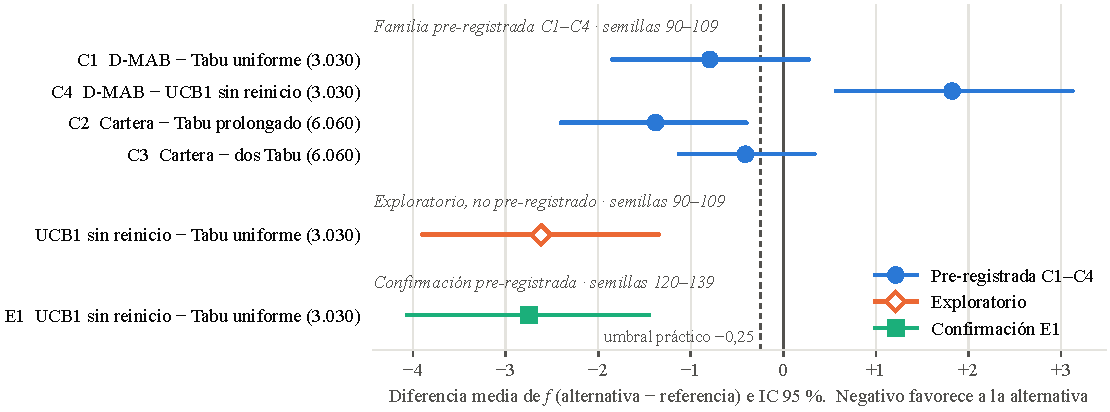
\includegraphics{figuras/forest_comparaciones}
 \caption{Diferencia media de $f$ e IC~95~\%; negativo favorece a la alternativa. Cada grupo es un análisis distinto.}
 \label{fig:forest}
\end{figure}

\subsection{La mejora de UCB1 cuesta cómputo y dispersión}
\label{subsec:costo}
Igual número de evaluaciones no significa igual cómputo. UCB1 repite más candidatos:
decodificó 10,1~\% más propuestas que Tabu uniforme y tardó 10,2~\% más (9,8~\%
en E1). D-MAB tardó 4,0~\% más.
% fuente: D (decoded_overhead, time_overhead)
UCB1 también fue más variable entre semillas, con DE de 9,36 frente a 8,72. En E1
se repitió el patrón: 9,89 frente a 8,90.
% fuente: D (sd)
La Figura~\ref{fig:distribucion} muestra que las distribuciones se superponen y que
la ventaja media de UCB1 se mantiene hasta el final.

En el piloto a igual tiempo, D-MAB fue peor que Tabu uniforme en tres de los cuatro
tamaños: $+0{,}21$, $-2{,}30$, $+2{,}70$ y $+6{,}00$. Son solo cinco semillas
por tamaño y el piloto no incluyó UCB1.
% fuente: R/entrega2_tiempo_110_114/summary.csv

\begin{figure}[!ht]
 \centering
 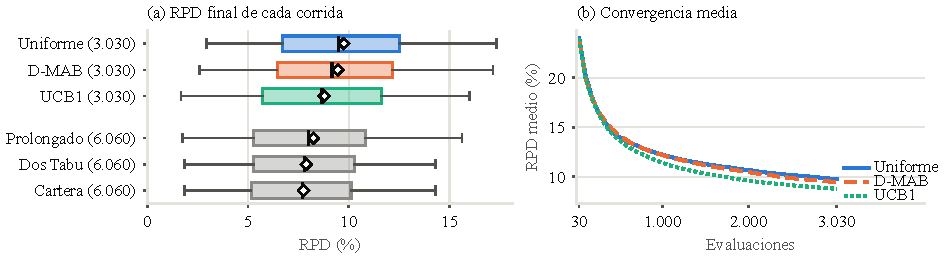
\includegraphics{figuras/distribucion_convergencia}
 \caption{Semillas 90--109. (a) RPD de 960 corridas por método: caja intercuartil, mediana, media (rombo) y percentiles 5--95. (b) RPD medio del mejor valor durante la búsqueda.}
 \label{fig:distribucion}
\end{figure}

\subsection{En el catálogo estándar los efectos no fueron consistentes}
\label{subsec:estandar}
Con la configuración vigente (semillas 40--59), los signos se invirtieron respecto
de la congestión. UCB1
menos uniforme dio $+1{,}182$; D-MAB menos uniforme, $+0{,}577$; y D-MAB menos
UCB1, $-0{,}605$.
% fuente: D (40-59)
Con la configuración anterior (semillas 20--39, $c=1$, $\lambda=0{,}35$), esas diferencias fueron
$-0{,}455$, $-0{,}513$ y $-0{,}058$.
% fuente: D (20-39)
En las semillas 60--79, D-MAB dio $+0{,}108$ frente a uniforme. La cartera dio
$-0{,}656$ frente al prolongado y $+0{,}134$ frente a dos Tabu.
% fuente: D (60-79)
Son descriptivos, con 12 instancias, y ninguno sustenta una superioridad.

\subsection{Discusión: bajo congestión ayuda UCB1, no el reinicio}
\label{subsec:discusion}
Los resultados responden la pregunta solo bajo escasez de cirujanos e igual número
de evaluaciones. Allí no identificamos una mejora concluyente de
D-MAB, mientras que UCB1 sí mejora, sobre todo desde 20 cirugías. La evidencia
señala al reinicio, con la configuración probada, como perjudicial en ese catálogo.
No demuestra que toda detección de cambios lo sea.

Una explicación plausible es que el detector confunde el agotamiento normal de la
búsqueda con un cambio entre operadores. Page--Hinkley detecta caídas de recompensa,
y las mejoras escasean al estancarse la búsqueda. D-MAB reinició una mediana de 24
veces por corrida, y cada reinicio borra sus estimaciones.
% fuente: R/entrega3_descriptivos/descriptivos.csv
La reparación no basta para explicarlo, porque afecta a todos. Alteró 46,6~\% de los
candidatos en uniforme, 44,0~\% en D-MAB y 40,1~\% en UCB1.
% fuente: R/entrega3_descriptivos/descriptivos.csv
Como no medimos si cambia el mejor operador, el mecanismo sigue siendo una hipótesis.

Este hallazgo concuerda con una parte de \textcite{dacosta2008}. En su escenario de
recompensas binarias, de alta varianza, el bandido sin reinicio superó a D-MAB.
Nuestra señal también es irregular: en el diagnóstico estándar, solo 3,9~\% de las
propuestas recibió recompensa positiva.
% fuente: R/entrega2_diagnostico_115_119/summary.csv
\textcite{dolatkhah2026} reinician con otra regla, una brecha entre operadores, por
lo que su resultado no valida este detector. \textcite{yin2026} miden brechas
frente a cotas; nuestro RPD, en cambio, no mide la distancia al óptimo.

E1 tampoco prueba que aprender sea la causa. UCB1 dedicó 39,1~\% de sus evaluaciones
al cambio de sala de anestesia, frente a 19,6~\% del uniforme.
% fuente: D (share_room_1)
Una mezcla fija con ese sesgo podría igualarlo. Además, confirmar con semillas
nuevas sobre las mismas instancias no mide generalización. Tampoco evaluamos
una cartera con UCB1.%
\label{res-fin}

% Cada cifra lleva su fuente en un comentario «% fuente: ruta».
% R = experiments/results. Las tablas y las figuras se generan con scripts.
% D = R/entrega3_revision/descriptivos.csv (descriptivo, no prerregistrado).
\section{Resultados y discusión}
\label{sec:resultados}\label{res-ini}
% Evita líneas viudas y huérfanas en esta sección y en la conclusión.
% \@clubpenalty es el valor que LaTeX restaura después de cada título.
\makeatletter\@clubpenalty=10000\makeatother
\clubpenalty=10000\widowpenalty=10000

\subsection{Tabu aporta la mayor parte de la mejora}
\label{subsec:absolutos}
El estudio completó los 960 pares sin fallos y su auditoría recalculó los 5.760
calendarios, todos factibles.
% fuente: R/entrega2_congestion_90_109/verification.json
El 51,8~\% de las soluciones de Tabu uniforme y D-MAB terminó con espera, entre
45,0~\% y 57,5~\% según el tamaño.
% fuente: R/entrega2_exploratorio/espera_por_tamano.csv
La Tabla~\ref{tab:descriptiva} muestra que Tabu uniforme ya mejora en 11,2~\% a la
mejor regla constructiva. UCB1 llega a 12,0~\%: cambiar la selección agrega menos de un
punto.
% fuente: D (improvement_over_best_rule)

\begin{table}[!ht]
 \centering
 \caption{Resultados en congestión (48 instancias, semillas 90--109; menor es mejor). RPD: respecto del mejor valor conocido, no del óptimo. Negrita: menor valor de cada bloque.}
 \label{tab:descriptiva}
 \scriptsize\setlength{\tabcolsep}{4pt}
 % Generado por experiments/scripts/tabla_descriptiva.py. No editar a mano.
% fuente: experiments/results/entrega3_revision/descriptivos.csv
\begin{tabular}{@{}lrrrrrrrrr@{}}
 \toprule
 & \multicolumn{5}{c}{Objetivo $f$ (unidades)} & \multicolumn{3}{c}{Componentes (min)} & \\
 \cmidrule(lr){2-6}\cmidrule(lr){7-9}
 Método & Mejor & Media & Peor & DE & RPD (\%) & $C_{\max}$ & $\sum W$ & $\max W$ & $t$ (s)\\
 \midrule
 FIFO & -- & 358,94 & -- & -- & 33,24 & 266,46 & 105,18 & 28,49 & --\\
 SPT & -- & 352,94 & -- & -- & 30,37 & 266,60 & 103,19 & 24,81 & --\\
 LPT & -- & 364,31 & -- & -- & 36,26 & 272,34 & 94,82 & 31,82 & --\\
 \midrule
 \multicolumn{10}{@{}l}{\emph{3.030 evaluaciones}}\\
 Uniforme & 280,31 & 297,20 & 312,80 & \textbf{8,72} & 9,75 & 287,56 & 9,31 & 3,55 & \textbf{6,17}\\
 D-MAB & 279,32 & 296,40 & 312,88 & 8,85 & 9,46 & 287,79 & 8,29 & 3,19 & 6,51\\
 UCB1 & \textbf{277,21} & \textbf{294,58} & \textbf{311,79} & 9,36 & \textbf{8,79} & \textbf{287,47} & \textbf{6,68} & \textbf{2,69} & 6,77\\
 \midrule
 \multicolumn{10}{@{}l}{\emph{6.060 evaluaciones}}\\
 Prolongado & 277,81 & 293,23 & 307,97 & 7,95 & 8,25 & 286,10 & \textbf{6,83} & \textbf{2,64} & \textbf{12,43}\\
 Dos Tabu & 277,87 & 292,26 & 305,89 & \textbf{7,29} & 7,89 & 284,74 & 7,16 & 2,81 & 12,59\\
 Cartera & \textbf{277,15} & \textbf{291,85} & \textbf{304,91} & \textbf{7,29} & \textbf{7,76} & \textbf{284,45} & 6,99 & 2,78 & 12,87\\
 \bottomrule
\end{tabular}

\end{table}

\subsection{La evidencia sobre D-MAB frente a Tabu uniforme no es concluyente}
\label{subsec:c1}
En C1 (Tabla~\ref{tab:comparaciones}), la diferencia media fue $-0{,}793$, con
IC~95~\% [$-1{,}850$; $+0{,}279$] y $p$ de Holm 0,041.
% fuente: R/entrega2_congestion_90_109/comparisons.csv (C1)
Wilcoxon rechaza la igualdad, pero el intervalo incluye el cero. Por tanto, la regla
prerregistrada no respalda la hipótesis primaria. El desacuerdo se relaciona con el
bootstrap: su error estándar es 1,62 veces el de las medias por instancia.
% fuente: D (bootstrap_se_ratio, C1)
Aunque es conservador, se fijó antes y no lo cambiamos.

El intervalo incluye beneficios y perjuicios mayores que el umbral de 0,25. Además,
la DE de las diferencias fue 13,21 y no la supuesta de 7,03. Así, la potencia para
detectar 0,65 cayó a 0,32, y el resultado no prueba equivalencia.
% fuente: R/entrega2_exploratorio/potencia_realizada.csv
La espera total bajó con D-MAB de 9,31 a 8,29 minutos. El \emph{makespan}, en
cambio, subió levemente, de 287,56 a 287,79.
% fuente: R/entrega2_congestion_90_109/descriptive.csv

\begin{table}[!ht]
 \centering
 \caption{Diferencias de $f$, en unidades del objetivo (semillas 90--109, 960 pares); negativo favorece a la alternativa. Negrita: cumple los tres criterios de la regla, que solo era vinculante para C1. Las columnas por tamaño son descriptivas, con 12 instancias cada una.}
 \label{tab:comparaciones}
 \scriptsize\setlength{\tabcolsep}{4pt}
 % Generado por experiments/scripts/tabla_resultados.py. No editar a mano.
% fuente: experiments/results/entrega2_congestion_90_109/comparisons.csv
% fuente de las columnas por tamaño: experiments/results/entrega3_revision/descriptivos.csv
\begin{tabular}{@{}llrcrrrrr@{}}
 \toprule
 & & & & & \multicolumn{4}{c}{Media por n.º de cirugías}\\
 \cmidrule(l){6-9}
 Id & Alternativa $-$ referencia & Media & IC 95~\% & $p$ Holm & 15 & 20 & 25 & 30\\
 \midrule
 \multicolumn{9}{@{}l}{\emph{3.030 evaluaciones por método}}\\
 C1 & D-MAB $-$ uniforme & $-0{,}793$ & [$-1{,}850$; $+0{,}279$] & $0{,}041$ & $-0{,}51$ & $-0{,}44$ & $-0{,}12$ & $-2{,}10$\\
 C4 & D-MAB $-$ UCB1 & $\mathbf{+1{,}824}$ & [$+0{,}566$; $+3{,}124$] & $0{,}005$ & $-0{,}98$ & $+1{,}40$ & $+4{,}95$ & $+1{,}93$\\
 \midrule
 \multicolumn{9}{@{}l}{\emph{6.060 evaluaciones por método}}\\
 C2 & Cartera $-$ prolongado & $\mathbf{-1{,}380}$ & [$-2{,}405$; $-0{,}398$] & $0{,}008$ & $+0{,}70$ & $+0{,}19$ & $-1{,}98$ & $-4{,}43$\\
 C3 & Cartera $-$ dos Tabu & $-0{,}409$ & [$-1{,}126$; $+0{,}338$] & $0{,}057$ & $-0{,}12$ & $-0{,}31$ & $+0{,}37$ & $-1{,}58$\\
 \bottomrule
\end{tabular}

\end{table}

\subsection{La cartera gana al prolongado, pero no a repetir la búsqueda}
\label{subsec:cartera}
La cartera superó al Tabu prolongado (C2), pero no se distinguió de dos Tabu
independientes (C3). Por tanto, no atribuimos su ganancia al aprendizaje. La
explicación más simple es el estancamiento. En 546 de las 960 corridas (56,9~\%),
el Tabu prolongado no mejoró después de la evaluación 3.030.
% fuente: R/entrega3_descriptivos/descriptivos.csv
La ventaja aparece con 25 y 30 cirugías; con 15 y 20, la cartera es peor en media.
Además, el error tipo~I simulado de C2 fue 0,082.
% fuente: R/entrega2_potencia/simulacion.csv

\subsection{UCB1 supera a D-MAB y a Tabu uniforme, según el tamaño}
\label{subsec:reinicio}
En C4, quitar el reinicio mejoró el resultado: con 25 cirugías, UCB1 venció a D-MAB
en las 12 instancias.
% fuente: D (instances_better_25, C4)
Con 15, en cambio, D-MAB fue mejor en media. El contraste exploratorio entre UCB1
y Tabu uniforme había dado $-2{,}617$.
% fuente: R/entrega2_exploratorio/contrastes.csv
Por eso, lo confirmamos con un protocolo propio y semillas nuevas. En E1, la
diferencia fue $-2{,}749$, con IC [$-4{,}069$; $-1{,}453$] y $p$ menor que 0,001
(Figura~\ref{fig:forest}).
% fuente: R/entrega3_confirmacion_ucb1/comparisons.csv (E1)

E1 cumple la regla y mejora en 38 de 48 instancias, pero equivale a solo 0,92~\%
de $f$. Además, depende del tamaño. Con 15, 20, 25 y 30 cirugías dio $+0{,}12$,
$-2{,}96$, $-3{,}91$ y $-4{,}25$: con 15 no hay ventaja.
% fuente: D (instances_better, relative_difference y difference_<tamaño>, E1)

\begin{figure}[!ht]
 \centering
 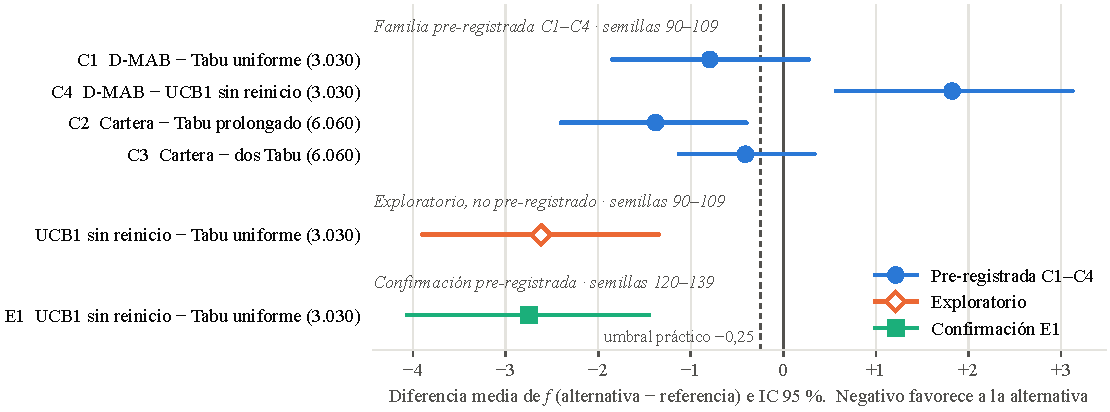
\includegraphics{figuras/forest_comparaciones}
 \caption{Diferencia media de $f$ e IC~95~\%; negativo favorece a la alternativa. Cada grupo es un análisis distinto.}
 \label{fig:forest}
\end{figure}

\subsection{La mejora de UCB1 cuesta cómputo y dispersión}
\label{subsec:costo}
Igual número de evaluaciones no significa igual cómputo. UCB1 repite más candidatos:
decodificó 10,1~\% más propuestas que Tabu uniforme y tardó 10,2~\% más (9,8~\%
en E1). D-MAB tardó 4,0~\% más.
% fuente: D (decoded_overhead, time_overhead)
UCB1 también fue más variable entre semillas, con DE de 9,36 frente a 8,72. En E1
se repitió el patrón: 9,89 frente a 8,90.
% fuente: D (sd)
La Figura~\ref{fig:distribucion} muestra que las distribuciones se superponen y que
la ventaja media de UCB1 se mantiene hasta el final.

En el piloto a igual tiempo, D-MAB fue peor que Tabu uniforme en tres de los cuatro
tamaños: $+0{,}21$, $-2{,}30$, $+2{,}70$ y $+6{,}00$. Son solo cinco semillas
por tamaño y el piloto no incluyó UCB1.
% fuente: R/entrega2_tiempo_110_114/summary.csv

\begin{figure}[!ht]
 \centering
 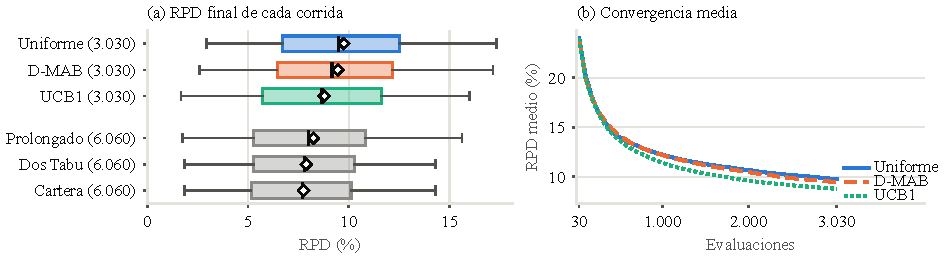
\includegraphics{figuras/distribucion_convergencia}
 \caption{Semillas 90--109. (a) RPD de 960 corridas por método: caja intercuartil, mediana, media (rombo) y percentiles 5--95. (b) RPD medio del mejor valor durante la búsqueda.}
 \label{fig:distribucion}
\end{figure}

\subsection{En el catálogo estándar los efectos no fueron consistentes}
\label{subsec:estandar}
Con la configuración vigente (semillas 40--59), los signos se invirtieron respecto
de la congestión. UCB1
menos uniforme dio $+1{,}182$; D-MAB menos uniforme, $+0{,}577$; y D-MAB menos
UCB1, $-0{,}605$.
% fuente: D (40-59)
Con la configuración anterior (semillas 20--39, $c=1$, $\lambda=0{,}35$), esas diferencias fueron
$-0{,}455$, $-0{,}513$ y $-0{,}058$.
% fuente: D (20-39)
En las semillas 60--79, D-MAB dio $+0{,}108$ frente a uniforme. La cartera dio
$-0{,}656$ frente al prolongado y $+0{,}134$ frente a dos Tabu.
% fuente: D (60-79)
Son descriptivos, con 12 instancias, y ninguno sustenta una superioridad.

\subsection{Discusión: bajo congestión ayuda UCB1, no el reinicio}
\label{subsec:discusion}
Los resultados responden la pregunta solo bajo escasez de cirujanos e igual número
de evaluaciones. Allí no identificamos una mejora concluyente de
D-MAB, mientras que UCB1 sí mejora, sobre todo desde 20 cirugías. La evidencia
señala al reinicio, con la configuración probada, como perjudicial en ese catálogo.
No demuestra que toda detección de cambios lo sea.

Una explicación plausible es que el detector confunde el agotamiento normal de la
búsqueda con un cambio entre operadores. Page--Hinkley detecta caídas de recompensa,
y las mejoras escasean al estancarse la búsqueda. D-MAB reinició una mediana de 24
veces por corrida, y cada reinicio borra sus estimaciones.
% fuente: R/entrega3_descriptivos/descriptivos.csv
La reparación no basta para explicarlo, porque afecta a todos. Alteró 46,6~\% de los
candidatos en uniforme, 44,0~\% en D-MAB y 40,1~\% en UCB1.
% fuente: R/entrega3_descriptivos/descriptivos.csv
Como no medimos si cambia el mejor operador, el mecanismo sigue siendo una hipótesis.

Este hallazgo concuerda con una parte de \textcite{dacosta2008}. En su escenario de
recompensas binarias, de alta varianza, el bandido sin reinicio superó a D-MAB.
Nuestra señal también es irregular: en el diagnóstico estándar, solo 3,9~\% de las
propuestas recibió recompensa positiva.
% fuente: R/entrega2_diagnostico_115_119/summary.csv
\textcite{dolatkhah2026} reinician con otra regla, una brecha entre operadores, por
lo que su resultado no valida este detector. \textcite{yin2026} miden brechas
frente a cotas; nuestro RPD, en cambio, no mide la distancia al óptimo.

E1 tampoco prueba que aprender sea la causa. UCB1 dedicó 39,1~\% de sus evaluaciones
al cambio de sala de anestesia, frente a 19,6~\% del uniforme.
% fuente: D (share_room_1)
Una mezcla fija con ese sesgo podría igualarlo. Además, confirmar con semillas
nuevas sobre las mismas instancias no mide generalización. Tampoco evaluamos
una cartera con UCB1.%
\label{res-fin}

% Cada cifra lleva su fuente en un comentario «% fuente: ruta».
% R = experiments/results. Las tablas y las figuras se generan con scripts.
% D = R/entrega3_revision/descriptivos.csv (descriptivo, no prerregistrado).
\section{Resultados y discusión}
\label{sec:resultados}\label{res-ini}
% Evita líneas viudas y huérfanas en esta sección y en la conclusión.
% \@clubpenalty es el valor que LaTeX restaura después de cada título.
\makeatletter\@clubpenalty=10000\makeatother
\clubpenalty=10000\widowpenalty=10000

\subsection{Tabu aporta la mayor parte de la mejora}
\label{subsec:absolutos}
El estudio completó los 960 pares sin fallos y su auditoría recalculó los 5.760
calendarios, todos factibles.
% fuente: R/entrega2_congestion_90_109/verification.json
El 51,8~\% de las soluciones de Tabu uniforme y D-MAB terminó con espera, entre
45,0~\% y 57,5~\% según el tamaño.
% fuente: R/entrega2_exploratorio/espera_por_tamano.csv
La Tabla~\ref{tab:descriptiva} muestra que Tabu uniforme ya mejora en 11,2~\% a la
mejor regla constructiva. UCB1 llega a 12,0~\%: cambiar la selección agrega menos de un
punto.
% fuente: D (improvement_over_best_rule)

\begin{table}[!ht]
 \centering
 \caption{Resultados en congestión (48 instancias, semillas 90--109; menor es mejor). RPD: respecto del mejor valor conocido, no del óptimo. Negrita: menor valor de cada bloque.}
 \label{tab:descriptiva}
 \scriptsize\setlength{\tabcolsep}{4pt}
 % Generado por experiments/scripts/tabla_descriptiva.py. No editar a mano.
% fuente: experiments/results/entrega3_revision/descriptivos.csv
\begin{tabular}{@{}lrrrrrrrrr@{}}
 \toprule
 & \multicolumn{5}{c}{Objetivo $f$ (unidades)} & \multicolumn{3}{c}{Componentes (min)} & \\
 \cmidrule(lr){2-6}\cmidrule(lr){7-9}
 Método & Mejor & Media & Peor & DE & RPD (\%) & $C_{\max}$ & $\sum W$ & $\max W$ & $t$ (s)\\
 \midrule
 FIFO & -- & 358,94 & -- & -- & 33,24 & 266,46 & 105,18 & 28,49 & --\\
 SPT & -- & 352,94 & -- & -- & 30,37 & 266,60 & 103,19 & 24,81 & --\\
 LPT & -- & 364,31 & -- & -- & 36,26 & 272,34 & 94,82 & 31,82 & --\\
 \midrule
 \multicolumn{10}{@{}l}{\emph{3.030 evaluaciones}}\\
 Uniforme & 280,31 & 297,20 & 312,80 & \textbf{8,72} & 9,75 & 287,56 & 9,31 & 3,55 & \textbf{6,17}\\
 D-MAB & 279,32 & 296,40 & 312,88 & 8,85 & 9,46 & 287,79 & 8,29 & 3,19 & 6,51\\
 UCB1 & \textbf{277,21} & \textbf{294,58} & \textbf{311,79} & 9,36 & \textbf{8,79} & \textbf{287,47} & \textbf{6,68} & \textbf{2,69} & 6,77\\
 \midrule
 \multicolumn{10}{@{}l}{\emph{6.060 evaluaciones}}\\
 Prolongado & 277,81 & 293,23 & 307,97 & 7,95 & 8,25 & 286,10 & \textbf{6,83} & \textbf{2,64} & \textbf{12,43}\\
 Dos Tabu & 277,87 & 292,26 & 305,89 & \textbf{7,29} & 7,89 & 284,74 & 7,16 & 2,81 & 12,59\\
 Cartera & \textbf{277,15} & \textbf{291,85} & \textbf{304,91} & \textbf{7,29} & \textbf{7,76} & \textbf{284,45} & 6,99 & 2,78 & 12,87\\
 \bottomrule
\end{tabular}

\end{table}

\subsection{La evidencia sobre D-MAB frente a Tabu uniforme no es concluyente}
\label{subsec:c1}
En C1 (Tabla~\ref{tab:comparaciones}), la diferencia media fue $-0{,}793$, con
IC~95~\% [$-1{,}850$; $+0{,}279$] y $p$ de Holm 0,041.
% fuente: R/entrega2_congestion_90_109/comparisons.csv (C1)
Wilcoxon rechaza la igualdad, pero el intervalo incluye el cero. Por tanto, la regla
prerregistrada no respalda la hipótesis primaria. El desacuerdo se relaciona con el
bootstrap: su error estándar es 1,62 veces el de las medias por instancia.
% fuente: D (bootstrap_se_ratio, C1)
Aunque es conservador, se fijó antes y no lo cambiamos.

El intervalo incluye beneficios y perjuicios mayores que el umbral de 0,25. Además,
la DE de las diferencias fue 13,21 y no la supuesta de 7,03. Así, la potencia para
detectar 0,65 cayó a 0,32, y el resultado no prueba equivalencia.
% fuente: R/entrega2_exploratorio/potencia_realizada.csv
La espera total bajó con D-MAB de 9,31 a 8,29 minutos. El \emph{makespan}, en
cambio, subió levemente, de 287,56 a 287,79.
% fuente: R/entrega2_congestion_90_109/descriptive.csv

\begin{table}[!ht]
 \centering
 \caption{Diferencias de $f$, en unidades del objetivo (semillas 90--109, 960 pares); negativo favorece a la alternativa. Negrita: cumple los tres criterios de la regla, que solo era vinculante para C1. Las columnas por tamaño son descriptivas, con 12 instancias cada una.}
 \label{tab:comparaciones}
 \scriptsize\setlength{\tabcolsep}{4pt}
 % Generado por experiments/scripts/tabla_resultados.py. No editar a mano.
% fuente: experiments/results/entrega2_congestion_90_109/comparisons.csv
% fuente de las columnas por tamaño: experiments/results/entrega3_revision/descriptivos.csv
\begin{tabular}{@{}llrcrrrrr@{}}
 \toprule
 & & & & & \multicolumn{4}{c}{Media por n.º de cirugías}\\
 \cmidrule(l){6-9}
 Id & Alternativa $-$ referencia & Media & IC 95~\% & $p$ Holm & 15 & 20 & 25 & 30\\
 \midrule
 \multicolumn{9}{@{}l}{\emph{3.030 evaluaciones por método}}\\
 C1 & D-MAB $-$ uniforme & $-0{,}793$ & [$-1{,}850$; $+0{,}279$] & $0{,}041$ & $-0{,}51$ & $-0{,}44$ & $-0{,}12$ & $-2{,}10$\\
 C4 & D-MAB $-$ UCB1 & $\mathbf{+1{,}824}$ & [$+0{,}566$; $+3{,}124$] & $0{,}005$ & $-0{,}98$ & $+1{,}40$ & $+4{,}95$ & $+1{,}93$\\
 \midrule
 \multicolumn{9}{@{}l}{\emph{6.060 evaluaciones por método}}\\
 C2 & Cartera $-$ prolongado & $\mathbf{-1{,}380}$ & [$-2{,}405$; $-0{,}398$] & $0{,}008$ & $+0{,}70$ & $+0{,}19$ & $-1{,}98$ & $-4{,}43$\\
 C3 & Cartera $-$ dos Tabu & $-0{,}409$ & [$-1{,}126$; $+0{,}338$] & $0{,}057$ & $-0{,}12$ & $-0{,}31$ & $+0{,}37$ & $-1{,}58$\\
 \bottomrule
\end{tabular}

\end{table}

\subsection{La cartera gana al prolongado, pero no a repetir la búsqueda}
\label{subsec:cartera}
La cartera superó al Tabu prolongado (C2), pero no se distinguió de dos Tabu
independientes (C3). Por tanto, no atribuimos su ganancia al aprendizaje. La
explicación más simple es el estancamiento. En 546 de las 960 corridas (56,9~\%),
el Tabu prolongado no mejoró después de la evaluación 3.030.
% fuente: R/entrega3_descriptivos/descriptivos.csv
La ventaja aparece con 25 y 30 cirugías; con 15 y 20, la cartera es peor en media.
Además, el error tipo~I simulado de C2 fue 0,082.
% fuente: R/entrega2_potencia/simulacion.csv

\subsection{UCB1 supera a D-MAB y a Tabu uniforme, según el tamaño}
\label{subsec:reinicio}
En C4, quitar el reinicio mejoró el resultado: con 25 cirugías, UCB1 venció a D-MAB
en las 12 instancias.
% fuente: D (instances_better_25, C4)
Con 15, en cambio, D-MAB fue mejor en media. El contraste exploratorio entre UCB1
y Tabu uniforme había dado $-2{,}617$.
% fuente: R/entrega2_exploratorio/contrastes.csv
Por eso, lo confirmamos con un protocolo propio y semillas nuevas. En E1, la
diferencia fue $-2{,}749$, con IC [$-4{,}069$; $-1{,}453$] y $p$ menor que 0,001
(Figura~\ref{fig:forest}).
% fuente: R/entrega3_confirmacion_ucb1/comparisons.csv (E1)

E1 cumple la regla y mejora en 38 de 48 instancias, pero equivale a solo 0,92~\%
de $f$. Además, depende del tamaño. Con 15, 20, 25 y 30 cirugías dio $+0{,}12$,
$-2{,}96$, $-3{,}91$ y $-4{,}25$: con 15 no hay ventaja.
% fuente: D (instances_better, relative_difference y difference_<tamaño>, E1)

\begin{figure}[!ht]
 \centering
 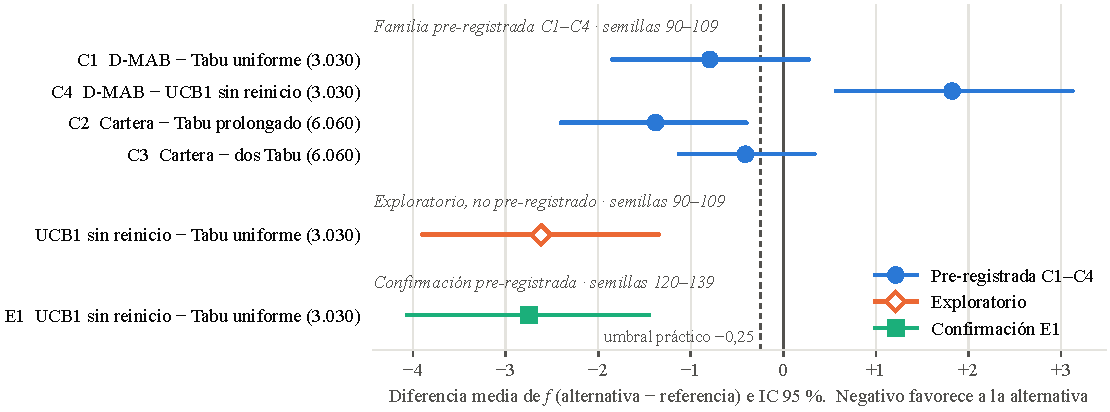
\includegraphics{figuras/forest_comparaciones}
 \caption{Diferencia media de $f$ e IC~95~\%; negativo favorece a la alternativa. Cada grupo es un análisis distinto.}
 \label{fig:forest}
\end{figure}

\subsection{La mejora de UCB1 cuesta cómputo y dispersión}
\label{subsec:costo}
Igual número de evaluaciones no significa igual cómputo. UCB1 repite más candidatos:
decodificó 10,1~\% más propuestas que Tabu uniforme y tardó 10,2~\% más (9,8~\%
en E1). D-MAB tardó 4,0~\% más.
% fuente: D (decoded_overhead, time_overhead)
UCB1 también fue más variable entre semillas, con DE de 9,36 frente a 8,72. En E1
se repitió el patrón: 9,89 frente a 8,90.
% fuente: D (sd)
La Figura~\ref{fig:distribucion} muestra que las distribuciones se superponen y que
la ventaja media de UCB1 se mantiene hasta el final.

En el piloto a igual tiempo, D-MAB fue peor que Tabu uniforme en tres de los cuatro
tamaños: $+0{,}21$, $-2{,}30$, $+2{,}70$ y $+6{,}00$. Son solo cinco semillas
por tamaño y el piloto no incluyó UCB1.
% fuente: R/entrega2_tiempo_110_114/summary.csv

\begin{figure}[!ht]
 \centering
 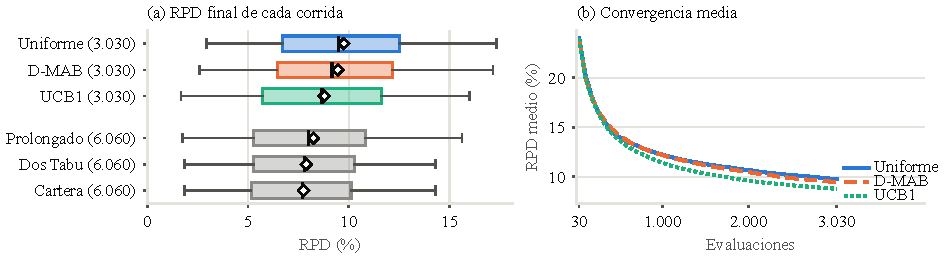
\includegraphics{figuras/distribucion_convergencia}
 \caption{Semillas 90--109. (a) RPD de 960 corridas por método: caja intercuartil, mediana, media (rombo) y percentiles 5--95. (b) RPD medio del mejor valor durante la búsqueda.}
 \label{fig:distribucion}
\end{figure}

\subsection{En el catálogo estándar los efectos no fueron consistentes}
\label{subsec:estandar}
Con la configuración vigente (semillas 40--59), los signos se invirtieron respecto
de la congestión. UCB1
menos uniforme dio $+1{,}182$; D-MAB menos uniforme, $+0{,}577$; y D-MAB menos
UCB1, $-0{,}605$.
% fuente: D (40-59)
Con la configuración anterior (semillas 20--39, $c=1$, $\lambda=0{,}35$), esas diferencias fueron
$-0{,}455$, $-0{,}513$ y $-0{,}058$.
% fuente: D (20-39)
En las semillas 60--79, D-MAB dio $+0{,}108$ frente a uniforme. La cartera dio
$-0{,}656$ frente al prolongado y $+0{,}134$ frente a dos Tabu.
% fuente: D (60-79)
Son descriptivos, con 12 instancias, y ninguno sustenta una superioridad.

\subsection{Discusión: bajo congestión ayuda UCB1, no el reinicio}
\label{subsec:discusion}
Los resultados responden la pregunta solo bajo escasez de cirujanos e igual número
de evaluaciones. Allí no identificamos una mejora concluyente de
D-MAB, mientras que UCB1 sí mejora, sobre todo desde 20 cirugías. La evidencia
señala al reinicio, con la configuración probada, como perjudicial en ese catálogo.
No demuestra que toda detección de cambios lo sea.

Una explicación plausible es que el detector confunde el agotamiento normal de la
búsqueda con un cambio entre operadores. Page--Hinkley detecta caídas de recompensa,
y las mejoras escasean al estancarse la búsqueda. D-MAB reinició una mediana de 24
veces por corrida, y cada reinicio borra sus estimaciones.
% fuente: R/entrega3_descriptivos/descriptivos.csv
La reparación no basta para explicarlo, porque afecta a todos. Alteró 46,6~\% de los
candidatos en uniforme, 44,0~\% en D-MAB y 40,1~\% en UCB1.
% fuente: R/entrega3_descriptivos/descriptivos.csv
Como no medimos si cambia el mejor operador, el mecanismo sigue siendo una hipótesis.

Este hallazgo concuerda con una parte de \textcite{dacosta2008}. En su escenario de
recompensas binarias, de alta varianza, el bandido sin reinicio superó a D-MAB.
Nuestra señal también es irregular: en el diagnóstico estándar, solo 3,9~\% de las
propuestas recibió recompensa positiva.
% fuente: R/entrega2_diagnostico_115_119/summary.csv
\textcite{dolatkhah2026} reinician con otra regla, una brecha entre operadores, por
lo que su resultado no valida este detector. \textcite{yin2026} miden brechas
frente a cotas; nuestro RPD, en cambio, no mide la distancia al óptimo.

E1 tampoco prueba que aprender sea la causa. UCB1 dedicó 39,1~\% de sus evaluaciones
al cambio de sala de anestesia, frente a 19,6~\% del uniforme.
% fuente: D (share_room_1)
Una mezcla fija con ese sesgo podría igualarlo. Además, confirmar con semillas
nuevas sobre las mismas instancias no mide generalización. Tampoco evaluamos
una cartera con UCB1.%
\label{res-fin}


\clearpage
% Sección (vi) Conclusión. Se inserta en main.tex después de Resultados y discusión:
%   \clearpage
%   % Sección (vi) Conclusión. Se inserta en main.tex después de Resultados y discusión:
%   \clearpage
%   % Sección (vi) Conclusión. Se inserta en main.tex después de Resultados y discusión:
%   \clearpage
%   \input{conclusion}
% No introduce cifras de resultados ni referencias nuevas: resume la sección anterior.
\section{Conclusión}
\label{sec:conclusion}\label{con-ini}

Este proyecto preguntó en qué condiciones D-MAB mejora Tabu Search frente a la
selección uniforme al programar cirugías en dos etapas. La literatura no había
medido ese aporte en un Tabu con espera estricta y reparación. Nuestra respuesta
es que no identificamos esa condición para D-MAB completo. Bajo congestión, el
resultado es no concluyente, porque el intervalo de la diferencia incluye el cero.

Sin embargo, el estudio deja tres hallazgos. Primero, la cartera supera al Tabu
prolongado con igual presupuesto. Segundo, esa ganancia es compatible con repetir
la búsqueda, porque no distinguimos la cartera de dos Tabu independientes.
Tercero, el reinicio Page--Hinkley no ayuda bajo congestión. De hecho, UCB1 sin
reinicio supera a D-MAB y, en una confirmación pre-registrada con semillas
nuevas, también a Tabu uniforme.

El aporte principal es metodológico. Diseñamos controles a igual presupuesto que
separan el aprendizaje del cómputo y de la repetición de la búsqueda. Además, dos
protocolos registrados antes de ejecutar restringieron nuestras decisiones. Así,
no declaramos un efecto que el intervalo no respalda, y confirmamos una señal
antes de afirmarla. Por último, generamos un catálogo de congestión que tensiona
la espera entre etapas.

Tres limitaciones acotan estas conclusiones. Primero, las semillas nuevas sobre
un mismo catálogo sintético no miden generalización a otros hospitales. Segundo,
la variabilidad observada dejó subdimensionada la comparación principal. Tercero,
comparamos por evaluaciones y en una sola máquina, no por tiempo.

Por tanto, el trabajo futuro debería contrastar cinco hipótesis. Primera: un
umbral $\lambda$ mayor reduce los reinicios y acerca D-MAB a UCB1. Segunda: un
crédito por rangos o por valores extremos entrega señal aunque las mejoras sean
escasas. Tercera: recompensar el movimiento aplicado, y no el propuesto, corrige
la distorsión de la reparación. Cuarta: reiniciar la búsqueda ante el
estancamiento reproduce la ganancia de la cartera. Quinta: un modelo sustituto
que prefiltre vecinos ahorra evaluaciones estrictas. Además, falta evaluar una
cartera con UCB1 frente a dos Tabu independientes. También faltan instancias
reservadas de 50 a 150 cirugías y una comparación a igual tiempo.

En conjunto, el proyecto muestra que el valor de un híbrido no depende de sumar
componentes de aprendizaje. Depende de comprobar, con controles, cuál de ellos
aporta. En este caso, aportó el componente más simple.
\label{con-fin}

% No introduce cifras de resultados ni referencias nuevas: resume la sección anterior.
\section{Conclusión}
\label{sec:conclusion}\label{con-ini}

Este proyecto preguntó en qué condiciones D-MAB mejora Tabu Search frente a la
selección uniforme al programar cirugías en dos etapas. La literatura no había
medido ese aporte en un Tabu con espera estricta y reparación. Nuestra respuesta
es que no identificamos esa condición para D-MAB completo. Bajo congestión, el
resultado es no concluyente, porque el intervalo de la diferencia incluye el cero.

Sin embargo, el estudio deja tres hallazgos. Primero, la cartera supera al Tabu
prolongado con igual presupuesto. Segundo, esa ganancia es compatible con repetir
la búsqueda, porque no distinguimos la cartera de dos Tabu independientes.
Tercero, el reinicio Page--Hinkley no ayuda bajo congestión. De hecho, UCB1 sin
reinicio supera a D-MAB y, en una confirmación pre-registrada con semillas
nuevas, también a Tabu uniforme.

El aporte principal es metodológico. Diseñamos controles a igual presupuesto que
separan el aprendizaje del cómputo y de la repetición de la búsqueda. Además, dos
protocolos registrados antes de ejecutar restringieron nuestras decisiones. Así,
no declaramos un efecto que el intervalo no respalda, y confirmamos una señal
antes de afirmarla. Por último, generamos un catálogo de congestión que tensiona
la espera entre etapas.

Tres limitaciones acotan estas conclusiones. Primero, las semillas nuevas sobre
un mismo catálogo sintético no miden generalización a otros hospitales. Segundo,
la variabilidad observada dejó subdimensionada la comparación principal. Tercero,
comparamos por evaluaciones y en una sola máquina, no por tiempo.

Por tanto, el trabajo futuro debería contrastar cinco hipótesis. Primera: un
umbral $\lambda$ mayor reduce los reinicios y acerca D-MAB a UCB1. Segunda: un
crédito por rangos o por valores extremos entrega señal aunque las mejoras sean
escasas. Tercera: recompensar el movimiento aplicado, y no el propuesto, corrige
la distorsión de la reparación. Cuarta: reiniciar la búsqueda ante el
estancamiento reproduce la ganancia de la cartera. Quinta: un modelo sustituto
que prefiltre vecinos ahorra evaluaciones estrictas. Además, falta evaluar una
cartera con UCB1 frente a dos Tabu independientes. También faltan instancias
reservadas de 50 a 150 cirugías y una comparación a igual tiempo.

En conjunto, el proyecto muestra que el valor de un híbrido no depende de sumar
componentes de aprendizaje. Depende de comprobar, con controles, cuál de ellos
aporta. En este caso, aportó el componente más simple.
\label{con-fin}

% No introduce cifras de resultados ni referencias nuevas: resume la sección anterior.
\section{Conclusión}
\label{sec:conclusion}\label{con-ini}

Este proyecto preguntó en qué condiciones D-MAB mejora Tabu Search frente a la
selección uniforme al programar cirugías en dos etapas. La literatura no había
medido ese aporte en un Tabu con espera estricta y reparación. Nuestra respuesta
es que no identificamos esa condición para D-MAB completo. Bajo congestión, el
resultado es no concluyente, porque el intervalo de la diferencia incluye el cero.

Sin embargo, el estudio deja tres hallazgos. Primero, la cartera supera al Tabu
prolongado con igual presupuesto. Segundo, esa ganancia es compatible con repetir
la búsqueda, porque no distinguimos la cartera de dos Tabu independientes.
Tercero, el reinicio Page--Hinkley no ayuda bajo congestión. De hecho, UCB1 sin
reinicio supera a D-MAB y, en una confirmación pre-registrada con semillas
nuevas, también a Tabu uniforme.

El aporte principal es metodológico. Diseñamos controles a igual presupuesto que
separan el aprendizaje del cómputo y de la repetición de la búsqueda. Además, dos
protocolos registrados antes de ejecutar restringieron nuestras decisiones. Así,
no declaramos un efecto que el intervalo no respalda, y confirmamos una señal
antes de afirmarla. Por último, generamos un catálogo de congestión que tensiona
la espera entre etapas.

Tres limitaciones acotan estas conclusiones. Primero, las semillas nuevas sobre
un mismo catálogo sintético no miden generalización a otros hospitales. Segundo,
la variabilidad observada dejó subdimensionada la comparación principal. Tercero,
comparamos por evaluaciones y en una sola máquina, no por tiempo.

Por tanto, el trabajo futuro debería contrastar cinco hipótesis. Primera: un
umbral $\lambda$ mayor reduce los reinicios y acerca D-MAB a UCB1. Segunda: un
crédito por rangos o por valores extremos entrega señal aunque las mejoras sean
escasas. Tercera: recompensar el movimiento aplicado, y no el propuesto, corrige
la distorsión de la reparación. Cuarta: reiniciar la búsqueda ante el
estancamiento reproduce la ganancia de la cartera. Quinta: un modelo sustituto
que prefiltre vecinos ahorra evaluaciones estrictas. Además, falta evaluar una
cartera con UCB1 frente a dos Tabu independientes. También faltan instancias
reservadas de 50 a 150 cirugías y una comparación a igual tiempo.

En conjunto, el proyecto muestra que el valor de un híbrido no depende de sumar
componentes de aprendizaje. Depende de comprobar, con controles, cuál de ellos
aporta. En este caso, aportó el componente más simple.
\label{con-fin}


\clearpage
\printbibliography[title={Referencias}]
\end{document}
